\section{Component Research}
This section discusses the extensive analysis our team took in order to choose the most optimum and efficient components available on the market. The first step took before choosing suitable components for our design was the research on what sensors could be useful in detecting the type of movements described earlier in this project. The initial sensors our team agreed on were accelerometers, gyroscopes and altimeters, taking into consideration the possibility that it would detect if the user is aboard an aircraft or not.

The main criteria on which we asserted the best component our design would need were: the working voltage, the current consumption, mounting type and if it was a multi-sensor component.
\begin{figure}
\centering
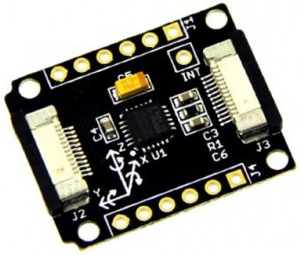
\includegraphics[scale=0.4]{figures/Xadow_IMU_6DOF.PNG}
\caption{Xadox IMU 6DOF Motion Tracker \label{fig:xadox}}
\end{figure}
After comparing various products from different suppliers, the final decision taken was ordering a motion tracking module based on the MPU6050, the Xadox IMU 6DOF Motion Tracker, which can be seen in figure \ref{fig:xadox} on the next page. It combines a 3-axis gyroscope, a 3-axis accelerometer and a Digital Motion Processor. This device offered the best compromise between current consumption and working voltage and at the point when we decided to order it. The team agreed that even if the accelerometer would offer the lowest current consumption, the gyroscope might give more accurate data results, it would be best to have a module which incorporates both.

